\chapter{}

%\begin{figure}[p]
%    \hspace*{-2.5cm}
%    \makebox[\linewidth]{
%        \setlength{\fboxsep}{0pt}
%        \fbox{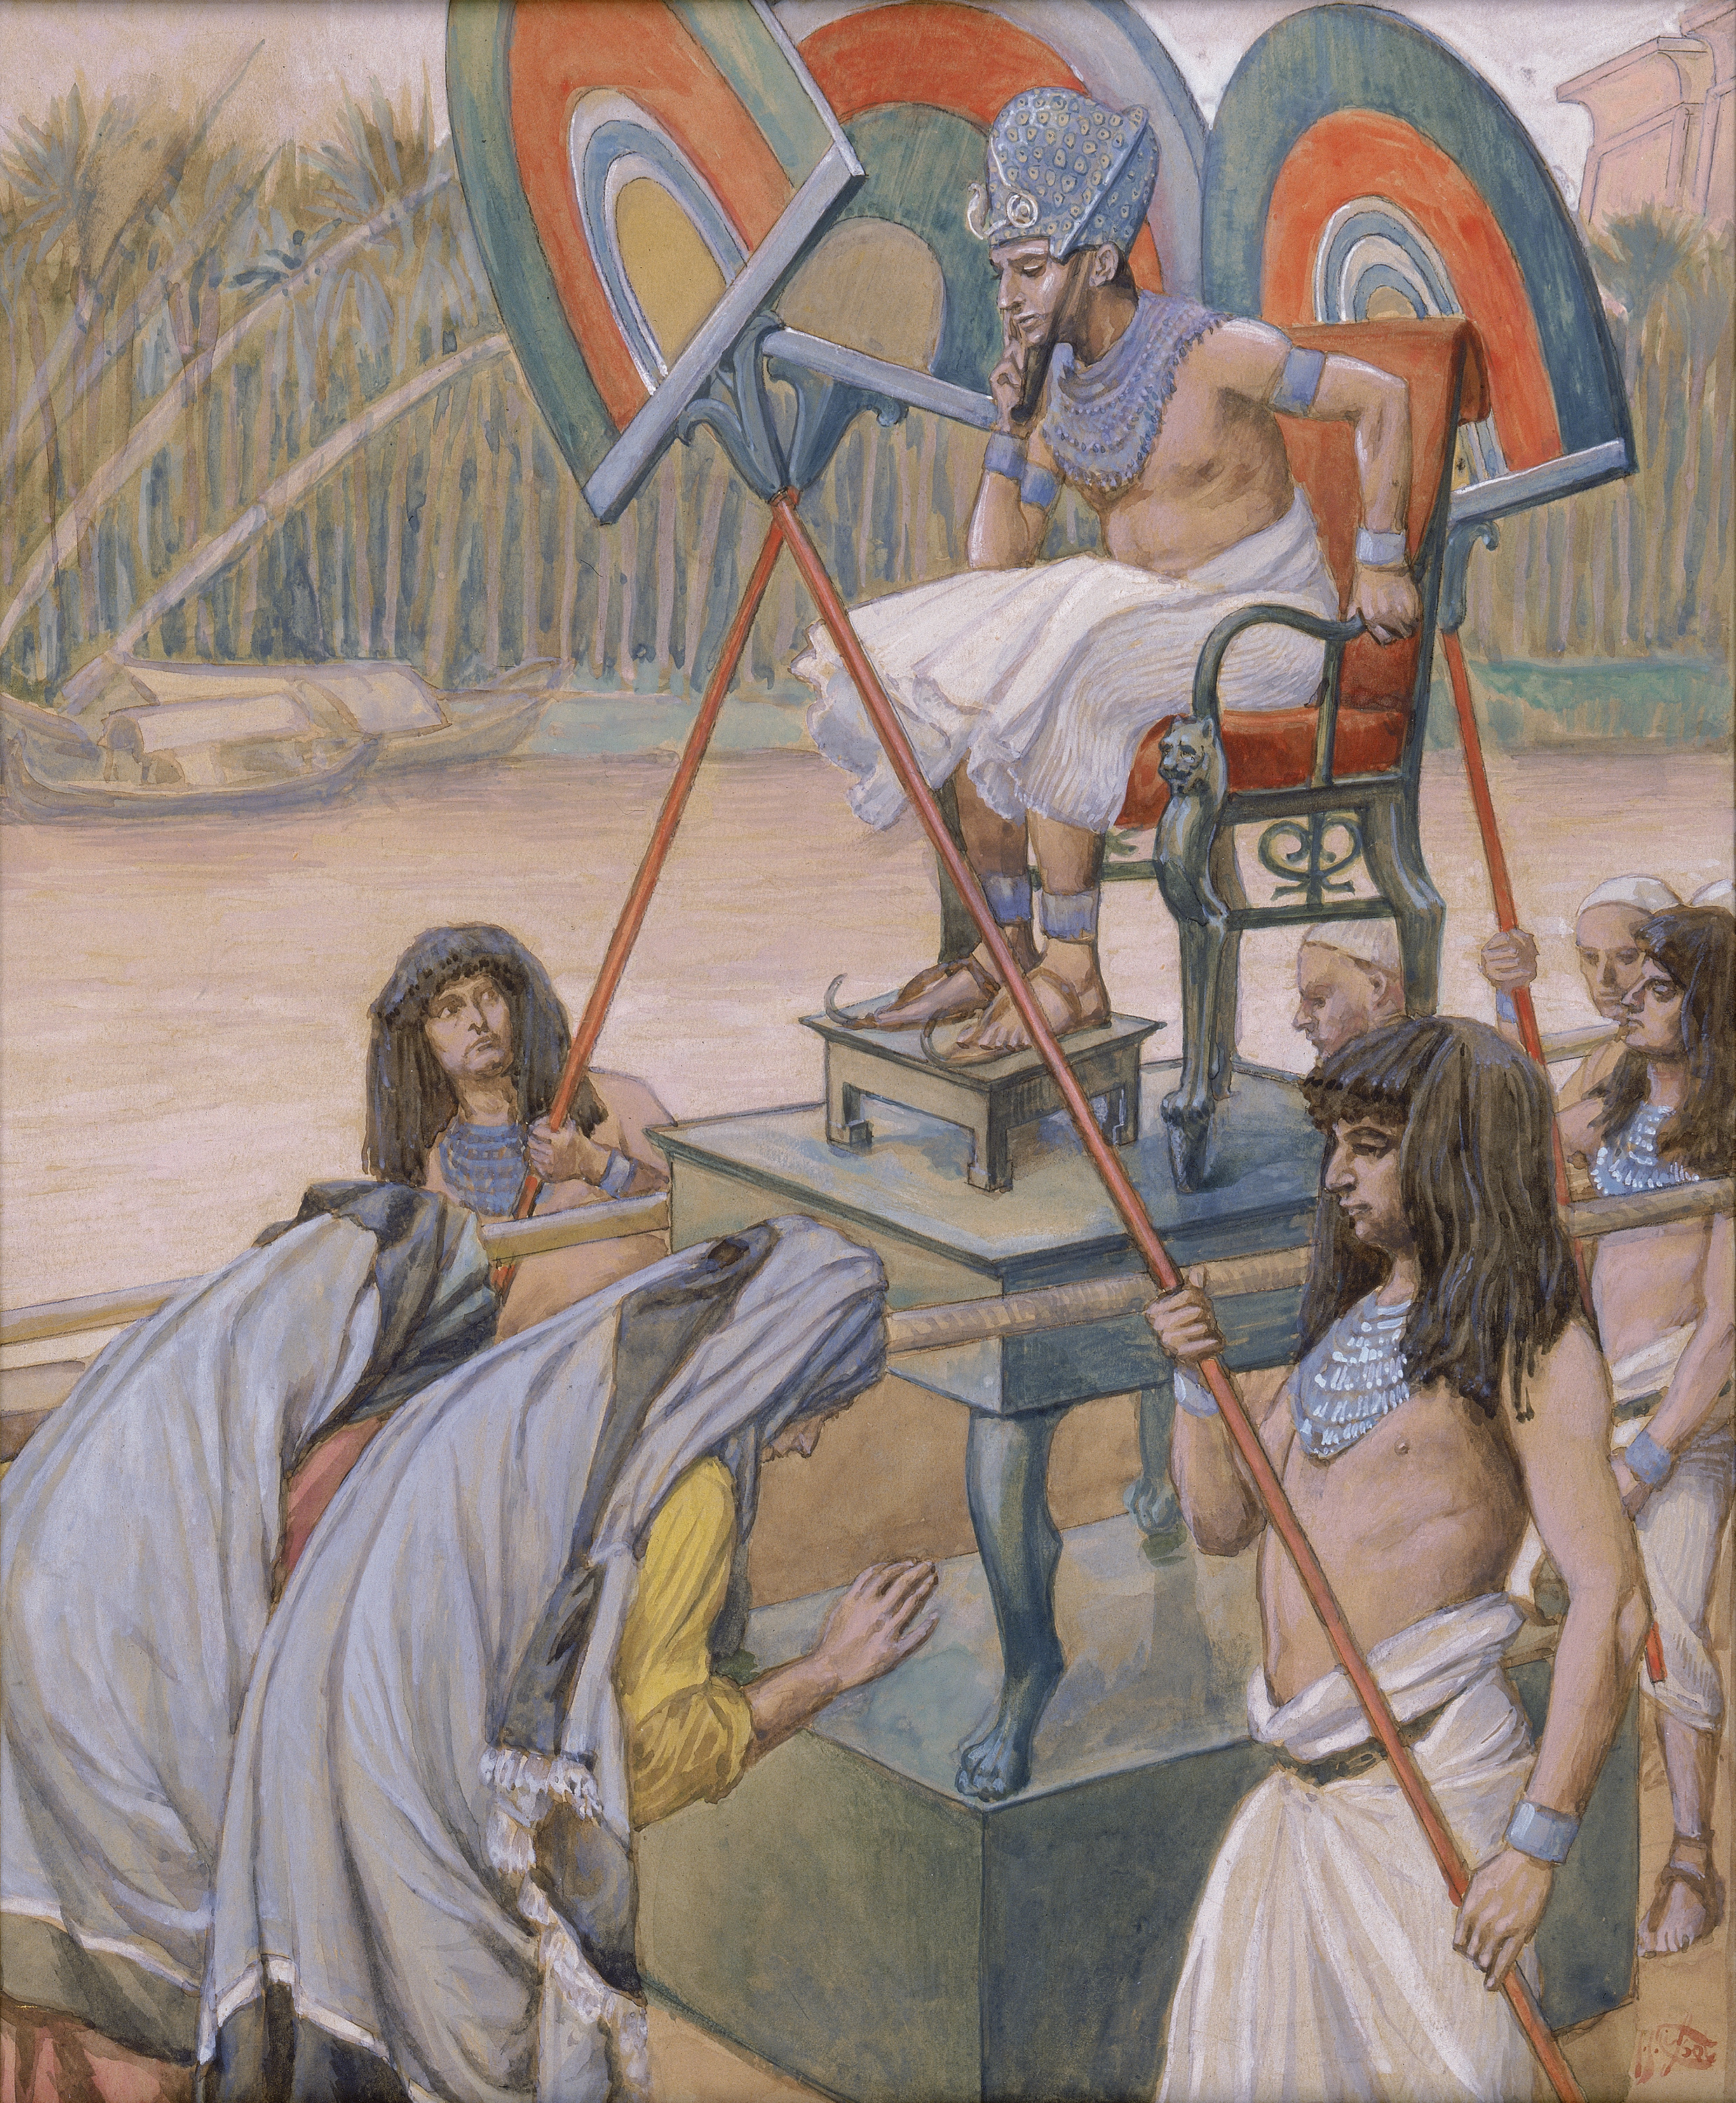
\includegraphics[width=1.3\linewidth]{midwives}}
%    }
%    \caption{\hspace*{-4.5cm}Obstetricēs et Rēx}
%\end{figure}

\titleimg{mw2.jpg}
\thispagestyle{empty}

\mktitle{Capitulum Primum}

\mpp{germināre:}{emittere germina (ea quae ex herbīs veniunt: semen, fructus, cēt.)}\mpp{quasi germinantēs:}{i.e, non vero germinantēs (quia hominēs non germinant) sed vidērī aliquō modō germināre}\cstart{F}{īliī} Isrāēl [in Ægyptō] crēvērunt, et quasi germinantēs \mpp{multiplicāre:}{multum facere; augēre}multiplicātī sunt:
ac rōborātī \mpp{rōborāre:}{virēs dāre}nimis, implēvērunt terram.

\vnum{8}Surrēxit intereā rēx novus super Ægyptum, quī ignōrābat Ioseph.
\vnum{9}Et ait ad populum suum: ``Ecce, populus fīliōrum Isrāēl multus, et fortior nōbīs est.
\vnum{10}Venīte, \mpp{sapienter (adv) <}{sapiēns}\mpp{opprimere:}{premere aliquem ne surgere possit}\mpp{ingruere:}{cum vi accedere}sapien\-ter opprimāmus eum, \mpp{ne forte...multiplicētur\\...addātur...egrediātur}{}nē forte multiplicētur: et sī ingruerit contrā nōs bellum, addātur inimīcīs nostrīs, expugnātisque nōbīs ēgrediātur dē terrā.''

\vnum{11}Præposuit itaque eīs magistrōs operum, ut \mpp{afflīgere:}{perturbāre, perdere}afflīgerent eōs oneribus: 
\mpp{onus, oneris (n):}{res quam difficile est portare vel agere. e.g: saccus lapidibus plenus, labor difficilis}ædificaveruntquē \mpp{urbēs tabernāculōrum:}{ubi rēs pretiosae regis et aliae rēs positae sunt}urbēs tabernāculōrum Pharaōnī, Phithom et Ramessēs.
\vnum{12}Quantōque opprimēbant eōs, tantō magis multiplicābantur, et crēscēbant: 
\vnum{13}ōderantque fīliōs Isrāēl Ægyptiī, et afflīgēbant \mpp{illūdere:}{deridēre}illūdentēs eīs,
\vnum{14}atque ad \mpp{amāritūdo, -inis (f)}{\\< amārus/a/um $\leftrightarrow$ dulcis, -e}amāritūdinem \mpp{per-dūcere:}{trahere}perdūcēbant vītam eōrum operibus dūrīs \mpp{lutum, -ī (n):}{terra humida}lutī et lateris, omnīque \mpp{famulātus, -ūs (m):}{servitūs}\mimg{later}{later, lateris (m)}famulātū, quō in terræ operibus premēbantur. 

\vnum{15}Dīxit autem rēx Ægyptī \mpp{obstetrix, -īcis (f):}{femina quae iuvat feminam gravidam parere} obstetrīcibus Hebræōrum, quārum ūna vocābātur Sephora, altera Phua, 
\mpp{praecipere:}{imperāre} \vnum{16}præcipiēns eīs: ``Quandō obstetrīcābitis Hebræās, et \mpp{partus, -ūs (m) <}{parere} partūs tempus advēnerit: sī masculus fuerit, interficite eum: sī fēmina, \mpp{reservāre:}{servāre, conservāre}reservātē.''

\vnum{17}Timuērunt autem obstetrīcēs Deum, \mpp{praeceptum, -ī:}{quod praecipitur}\mpp{nōn fēcērunt iuxtā praeceptum regis:}{nōn pāruērunt praeceptō rēgis}et nōn fēcērunt iuxtā præceptum rēgis Ægyptī, sed \mpp{cōnservāre:}{servāre}cōnservābant \mpp{mas, maris (m):}{homo (vel animal) masculinus}marēs. 
\vnum{18}Quibus ad sē accersītis, rēx ait: ``Quidnam est hoc quod facere voluistis, ut puerōs servārētis?''

\vnum{19}Quæ respondērunt: ``Nōn sunt Hebreæ sīcut Ægyptiæ mulierēs: ipsæ enim obstetrīcandī habent \mpp{scientia, -ae (f):}{id quod scītur}scientiam, et priusquam veniāmus ad eās, pariunt.''

\vnum{20}Bene ergō fēcit Deus obstetrīcibus: et crēvit populus, \mpp{cōnfortāre:}{fortem facere, consolārī}cōnfortātusque est nimis.
\vnum{21}Et quia timuērunt obstetrīcēs Deum, ædificāvit eīs domōs.
\vnum{22}Præcēpit ergō Pharaō omnī populō suō, dīcēns: ``Quidquid masculīnī sexūs nātum fuerit, in flūmen prōicite: quidquid fēminīnī, reservātē.''
